\phantomsection
\chapter{Results}
\label{chap:eval_results}

\noindent Two kinds of results have been obtained. First results have been obtained by using a test set from the database used for the training set. The LBP operator extracts features from each image of the test set, then classification is performed. The second result set is obtained with the Kinect. The Kinect gets video sequences of a subject in front of the Kinect and his or her face is extracted from these sequences. Then the same feature extraction and classification process is applied to these images.
\newline

\phantomsection
\section{First result set}

\vspace{\baselineskip}
\noindent To train the model, 128 face images from the KDEF database have been used for each emotion, plus neutral state. In total, $ 128\times7 = 896 $ face images have been used to train the model. To test the model, 12 face images from the KDEF database have been used for each emotion, plus neutral state. In total, $ 12\times7 = 84 $ faces images have been used to test the model. For each of these 84 images, face detection was used first, then LBP operator to extract features, and then classification using SVM.
\newline

\noindent For the classification part, the model has been trained with different kernels and different parameters. The results of this process are summed up in the table~\ref{table_results_kernels}.
\newline

\begin{table}[h]
   \caption{\label{table_results_kernels} Results with different kernels and different parameters}
   \begin {center}
\begin{tabular}{|c|c|c|c|c|c|c|c|c|}
  \hline
    & Linear & Poly1 & Poly2 & RBF1 & RBF2 & Sigmoid1 & Sigmoid2 \\
  \hline
  neutral & 33.33\% & 33.33\% & 25.00\% & 33.33\% & 33.33\% & 58,33\% & 41.67\% \\
  afraid & 66.67\% & 91.67\% & 100.00\% & 75.00\% & 83.33\% & 75.00\% & 75.00\% \\
  angry & 50.00\% & 50.00\% & 41.67\% & 50.00\% & 50.00\% & 66.67\% & 50.00\% \\
  disgusted & 75.00\% & 83.33\% & 83.33\% & 75.00\% & 75.00\% & 75.00\% & 83.33\% \\
  happy & 91.67\% & 91.67\% & 91.67\% & 91.67\% & 91.67\% & 91.67\% & 91.67\% \\
  sad & 16.67\% & 16.67\% & 8.33\% & 8.33\% & 8.33\% & 8.33\% & 16.67\% \\
  surprised & 33.33\% & 58.33\% & 50.00\% & 66.67\% & 58.33\% & 50.00\% & 75.00\% \\
  overall & 52.38\% & 60.71\% & 57.14\% & 57.14\% & 57.14\% & 60.71\% & 61.90\% \\
  \hline
\end{tabular}
\end {center}
\end{table}

\noindent Poly1 stands for Polynomial and has degree parameter: $ D = 2 $
\newline
\noindent Poly2 stands for Polynomial and has degree parameter: $ D = 3 $
\newline
\noindent RBF1 has cache and $\gamma$ parameters: $ C = 8.0 $ and $ \gamma = 0.0078125 $
\newline
\noindent RBF2 has cache and $\gamma$ parameters: $ C = 32.0 $ and $ \gamma = 0.001953125 $ 
\newline
\noindent Sigmoid1 has cache and $\gamma$ parameters: $ C = 8.0 $ and $ \gamma = 0.0078125 $
\newline
\noindent Sigmoid2 has cache and $\gamma$ parameters: $ C = 32.0 $ and $ \gamma = 0.001953125 $
\newline

\noindent The same data has been trained with the same kernels and parameters but using cross-validation (as explained in Chapter \ref{chap:implementation_svm}). All results are inferior or equal to those without cross-validation, except for the linear kernel. The table~\ref{table_results_crossvalidation} represents both results with and without cross validation.
\newline

\begin{table}[h]
   \caption{\label{table_results_crossvalidation} Results with and without cross validation}
\begin {center}
\begin{tabular}{|c|c|c|c|c|c|c|c|c|}
  \hline
    & with cross validation & without cross validation \\
  \hline
  Linear & 53.57\% & 52.38\% \\
  Poly1 & 54.76\% & 60.71\% \\
  Poly2 & 44.05\% & 57.14\% \\
  RBF1 & 55.95\% & 57.14\% \\
  RBF2 & 50.00\% & 57.14\% \\
  Sigmoid1 & 55.95\% & 60.71\% \\
  Sigmoid2 & 61.90\% & 61.90\% \\
  \hline
\end{tabular}
\end {center}
\end{table}

\noindent The best accuracy percentage is for the Sigmoid2 kernel parameters. It is obtained with a classification based on the Sigmoid kernel and with following parameters: $ C = 32.0 $ and $ \gamma = 0.001953125 $. These parameters are found by \textit{gridsearch}, a script of the SVM library. They are the most optimized for the RBF kernel and for the Sigmoid kernel. The overall percentage of accuracy for all the emotions is $ 61.90\% $. The table~\ref{table_results_confusion_matrix} represents the confusion matrix.
\newline

\begin{table}[h]
   \caption{\label{table_results_confusion_matrix} Confusion matrix}
\begin {center}
\begin{tabular}{|c|c|c|c|c|c|c|c|c|}
  \hline
   & neutral & afraid & angry & disgusted & happy & sad & surprised & accuracy \\
  \hline
  neutral & 5 & 4 & 2 & 0 & 1 & 0 & 0 & 41.67\% \\
  afraid & 0 & 9 & 0 & 0 & 0 & 2 & 1 & 75.00\% \\
  angry & 2 & 3 & 6 & 0 & 0 & 1 & 0 & 50.00\% \\
  disgusted & 0 & 1 & 0 & 10 & 0 & 1 & 0 & 83.33\% \\
  happy & 0 & 0 & 0 & 1 & 11 & 0 & 0 & 91.67\% \\
  sad & 0 & 4 & 3 & 1 & 2 & 2 & 0 & 16.67\% \\
  surprised & 2 & 1 & 0 & 0 & 0 & 0 & 9 & 75.00\%\\
  \hline
\end{tabular}
\end {center}
\end{table}

\noindent By looking at the confusion matrix, it is easy to notice that 3 facial expressions are harder to recognize than the others with this system: angry, sad and neutral. There is a great difference between these 3 emotions and the 4 other ones (afraid, disgusted, happy and surprised). Indeed, these 3 emotions are recognized with an accuracy lower than $ 50\% $, while the 4 other ones are recognized with an accuracy higher than $ 70\% $. Furthermore, the recognition accuracy for the "Sad" expression is lower than random guess. The table~\ref{table_results_accuracy} shows the recognition accuracy of the six basic emotions and of the neutral state.
\newline

\begin{table}[h]
   \caption{\label{table_results_accuracy} Recognition accuracy of the six basic emotions and of the neutral state}
\begin {center}
\begin{tabular}{|c|c|c|c|c|c|c|c|c|}
  \hline
   $ < 50\% $ & > 75\% \\
  \hline
  neutral ($ 5/12 $) & afraid ($ 9/12 $) \\
  angry ($ 6/12 $) & disgusted ($ 10/12 $) \\
  sad ($ 2/12 $) & happy ($ 11/12 $) \\
   & surprised ($ 9/12 $) \\
  \hline
\end{tabular}
\end {center}
\end{table}

\noindent The numbers in parenthesis represent the number of faces correctly classified over the total number of face images tested.
\newline

\noindent These 6 emotions plus the neutral state can be categorized into 2 groups. Indeed, one group containing the 3 emotions hard to recognize and a second group containing the 4 remaining emotions. The 3 facial expressions \textit{angry}, \textit{sad} and \textit{neutral}, are the ones that distort the less the face. For a same subject expressing these 3 different emotions, as in Figure \ref{kdef_no_difference_emotions}, the differences are not clearly noticeable.
\newline

\begin{figure}[!h]
\begin{center}
\noindent 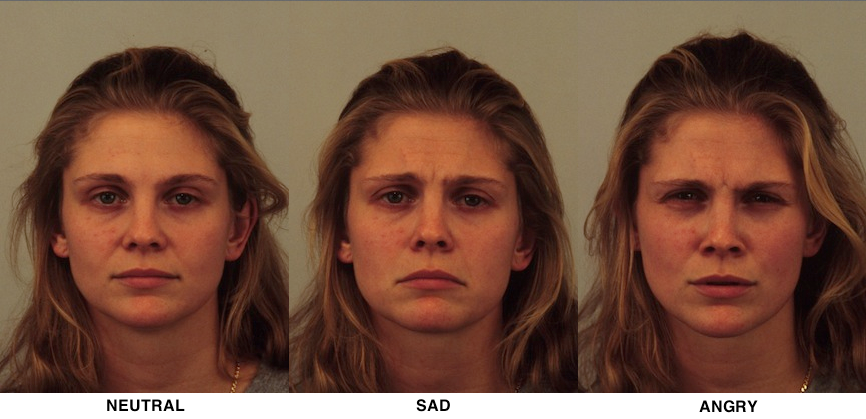
\includegraphics[scale=0.4]{figures/kdef_no_difference_emotions} 
\newline
\caption{Face images from the KDEF database used in the test set}
\label{kdef_no_difference_emotions}
\end{center} 
\end{figure}

\noindent The second group contains the 4 following facial expressions \textit{afraid}, \textit{disgusted}, \textit{happy} and \textit{surprised}. These emotions distort significantly the face when they are expressed. This is why it is easier to recognize them. Figure~\ref{kdef_difference_emotions} shows face images from the KDEF database used in the test set, expressing these 4 facial expressions. Important features carrying emotion as the mouth or the eyes are changing a lot while these 4 emotions are expressed.
\newline

\begin{figure}[!h]
\begin{center}
\noindent 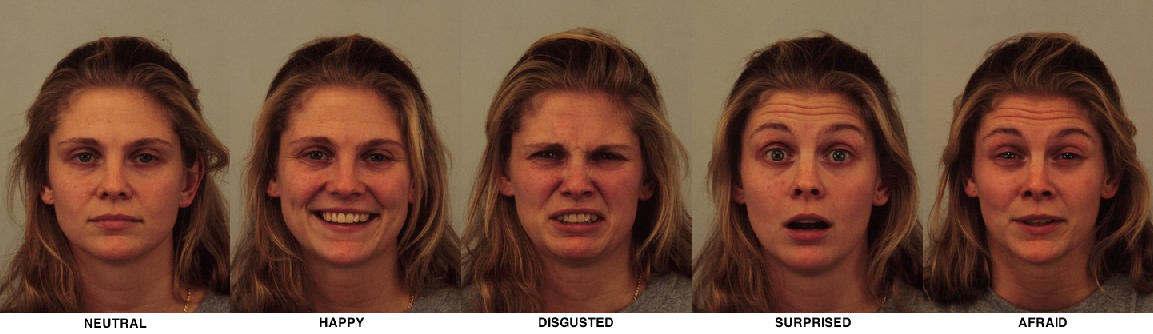
\includegraphics[scale=0.3]{figures/kdef_difference_emotions} 
\newline
\caption{Face images from the KDEF database used in the test set}
\label{kdef_difference_emotions}
\end{center} 
\end{figure}

\noindent As it can be seen in Figure~\ref{kdef_difference_emotions}, for each emotion, eyebrows are raised, eyes are widely opened, and the mouth has a distinct shape, whereas in Figure~\ref{kdef_no_difference_emotions} there are no differences as visible as in Figure~\ref{kdef_difference_emotions}. These variations of intensity might explain twhy the system struggles when trying to differentiate \textit{angry}, \textit{sad} and \textit{neutral} emotional states.
\newline

\phantomsection
\section{Second result set}

\vspace{\baselineskip}
\noindent The second result test is obtained based on the same process than the process that gives the first result set, the only difference being the input. Indeed, it is not images from which features are then extracted; it is a video stream from the Kinect. A subject stands in face of the Kinect, face is detected and extracted, then features are computed, and finally classification is performed. It runs almost in real-time, and the output is the name of the emotion expressed.
\newline

\subsection{With face images from the KDEF database}

\vspace{\baselineskip}
\noindent Because the results do not have a good accuracy at first sight, another method is tested. Face images from the KDEF database are printed on A4 paper and are put in front of the Kinect.
\newline

\noindent GIVE THE RESULTS OBTAINED
\newline

\subsection{With subjects}

\vspace{\baselineskip}
\noindent GIVE THE RESULTS OBTAINED
\newline

